\documentclass[12pt]{article}
\usepackage{graphicx}
\title{Práctica 2: Problemas con redes de Hopfield}
\author{Manuel González González}
\begin{document}
\maketitle
\section*{Ejercicio 2}
\subsection*{a)}
Encuentra un mínimo global porque no existen combinaciones con menor energía posible.
\subsection*{b)}
difEnergia = E-Eprev;
\subsection*{c)}
No se ejecutará ninguna vez ya que la energía o se queda igual (dejando el diferencial a cero) o disminuye (dejando el diferencial negativo).

\section*{Ejercicio 3}
\subsection*{a)}
No, se queda oscilando entre dos estados.
\subsection*{b)}
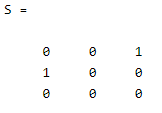
\includegraphics[scale=2]{primeraparalela.png}
\subsection*{c)}
La matriz no es semidefinida positiva. A la izquierda se puede ver el código ejecutado; a la derecha al matriz de pesos resultante; y debajo el resultado de la ejecución.\\
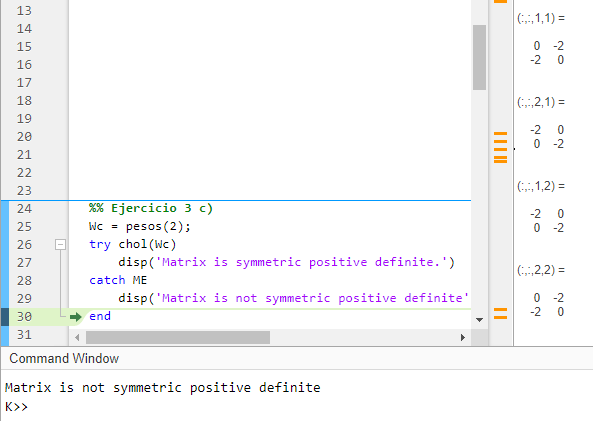
\includegraphics[scale=1]{paralelados.png}

\section*{Ejercicio 4}
\subsection*{a)}
Sí, se activa.

\subsection*{b)}
Se estabiliza en\\
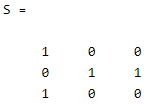
\includegraphics[scale=2]{cuatroejec.png}

\subsection*{c)}
Es un m\'inimo local, porque no es la soluci\'on \'optima del problema y no es capaz de cambiar de estado para encontrar otra.

\subsection*{d)}
En lugar de activar la unidad si el potencial sin\'aptico es mayor o igual al sesgo lo har\'ia solo si es mayor a este.

\section*{Ejercicio 5}
\subsection*{a)}
El tiempo medio para 100 ejecuciones con 3 torres es de $3'9e^{-4}$ segundos.
\subsection*{b)}
El tiempo medio para 100 ejecuciones con 30 torres es de $9'2e^{-3}$ segundos.
\subsection*{c)}
No se mantiene. La proporci\'on deber\'ia ser 10 veces mayor, pero es 20 veces mayor.\\
 
\end{document}